%% fig_simplextype.tex   (generated by make_round22.py; do not edit by hand)
%% The Klein quartic x^3y + y^3z + z^3x (thm:simplextype): its Newton triangle, of normalised area 7 with three interior points, and a smooth fan adapted to it.
\documentclass[tikz,border=8pt]{standalone}
\usepackage{amsmath,amssymb}
\usetikzlibrary{arrows.meta,calc,decorations.pathreplacing}
%% palette.tex -- shared colour definitions for the figures
\definecolor{PInk}{RGB}{26,32,44}
\definecolor{PBlue}{RGB}{37,82,139}
\definecolor{PTeal}{RGB}{23,127,125}
\definecolor{POchre}{RGB}{193,138,44}
\definecolor{PClay}{RGB}{178,74,58}
\definecolor{PSlate}{RGB}{108,122,137}
\definecolor{PViolet}{RGB}{110,86,150}
\definecolor{WBlue}{RGB}{223,234,246}
\definecolor{WTeal}{RGB}{220,238,236}
\definecolor{WOchre}{RGB}{250,240,218}
\definecolor{WClay}{RGB}{247,229,224}
\definecolor{WSlate}{RGB}{238,241,244}
\definecolor{PMag}{RGB}{158,58,110}
\definecolor{PGrass}{RGB}{62,124,66}
\definecolor{PAmber}{RGB}{214,112,38}
\definecolor{PIndigo}{RGB}{58,64,140}
\definecolor{PRule}{RGB}{176,186,197}

%% shared macros so the standalone figures match the paper
\providecommand{\QQ}{\mathbb{Q}}
\providecommand{\ZZ}{\mathbb{Z}}
\providecommand{\RR}{\mathbb{R}}
\providecommand{\CC}{\mathbb{C}}
\providecommand{\PP}{\mathbb{P}}
\providecommand{\Kx}{K^{\times}}
\providecommand{\HW}{W}
\providecommand{\Nm}{\mathrm{N}}
\providecommand{\Hdg}{\mathrm{Hdg}}
\providecommand{\NS}{\mathrm{NS}}
\providecommand{\cA}{\mathcal{A}}
\providecommand{\cD}{\mathcal{D}}
\providecommand{\cF}{\mathcal{F}}
\providecommand{\cP}{\mathcal{P}}
\providecommand{\cO}{\mathcal{O}}
\providecommand{\cQ}{\mathcal{Q}}
\providecommand{\bbar}[1]{\overline{#1}}
\providecommand{\ch}{\operatorname{ch}}
\providecommand{\End}{\mathrm{End}}
\providecommand{\Ext}{\operatorname{Ext}}
\providecommand{\Supp}{\operatorname{Supp}}

\begin{document}
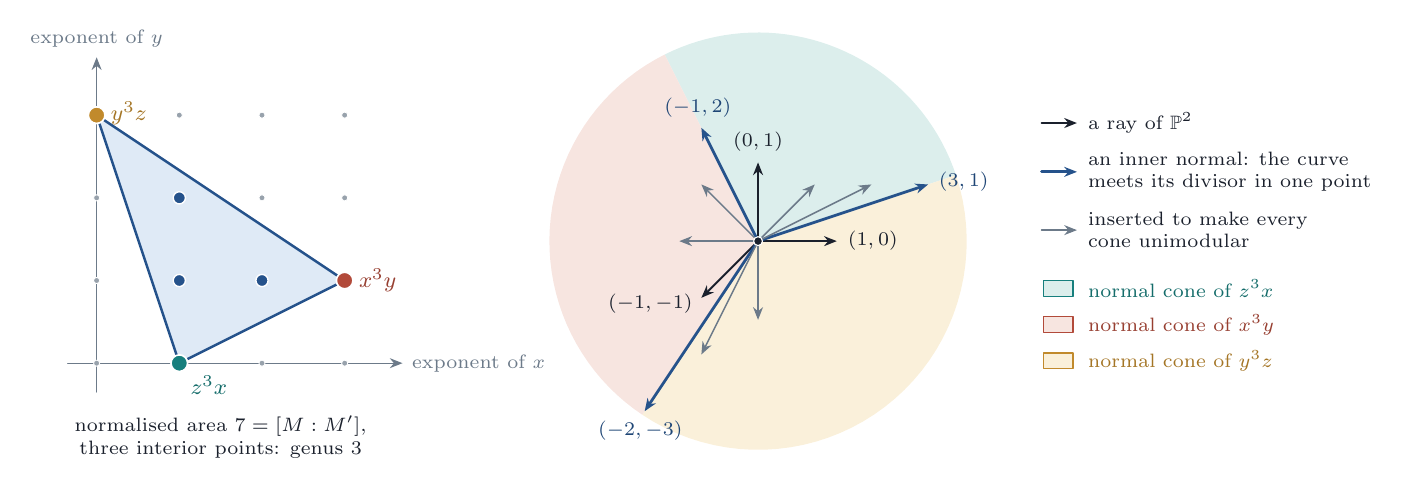
\begin{tikzpicture}[x=1cm,y=1cm,line join=round,line cap=round,
  font=\small,text=PInk,lbl/.style={inner sep=1pt}]
  \path[fill=WBlue,draw=PBlue,line width=0.90pt] (1.0500,0.0000) -- (3.1500,1.0500) -- (0.0000,3.1500) -- cycle;
  \path[fill=WTeal,draw=none] (8.4000,1.5500) -- (10.9140,2.3880) -- (10.8758,2.4948) -- (10.8331,2.6000) -- (10.7860,2.7031) -- (10.7344,2.8042) -- (10.6786,2.9030) -- (10.6186,2.9993) -- (10.5545,3.0929) -- (10.4865,3.1837) -- (10.4146,3.2715) -- (10.3391,3.3562) -- (10.2600,3.4375) -- (10.1775,3.5154) -- (10.0918,3.5897) -- (10.0029,3.6603) -- (9.9111,3.7269) -- (9.8165,3.7896) -- (9.7194,3.8482) -- (9.6198,3.9026) -- (9.5180,3.9526) -- (9.4141,3.9983) -- (9.3084,4.0394) -- (9.2010,4.0760) -- (9.0921,4.1080) -- (8.9820,4.1353) -- (8.8708,4.1578) -- (8.7588,4.1756) -- (8.6460,4.1886) -- (8.5329,4.1967) -- (8.4195,4.1999) -- (8.3060,4.1983) -- (8.1927,4.1919) -- (8.0798,4.1806) -- (7.9675,4.1645) -- (7.8560,4.1436) -- (7.7455,4.1179) -- (7.6362,4.0875) -- (7.5283,4.0525) -- (7.4220,4.0129) -- (7.3174,3.9688) -- (7.2149,3.9202) -- cycle;
  \path[fill=WClay,draw=none] (8.4000,1.5500) -- (7.2149,3.9202) -- (7.0927,3.8551) -- (6.9741,3.7837) -- (6.8594,3.7062) -- (6.7489,3.6228) -- (6.6429,3.5337) -- (6.5417,3.4392) -- (6.4456,3.3396) -- (6.3548,3.2351) -- (6.2696,3.1260) -- (6.1902,3.0126) -- (6.1168,2.8952) -- (6.0497,2.7741) -- (5.9889,2.6497) -- (5.9348,2.5223) -- (5.8874,2.3922) -- (5.8468,2.2598) -- (5.8133,2.1255) -- (5.7867,1.9896) -- (5.7673,1.8526) -- (5.7551,1.7147) -- (5.7501,1.5763) -- (5.7524,1.4379) -- (5.7618,1.2998) -- (5.7785,1.1623) -- (5.8023,1.0260) -- (5.8332,0.8910) -- (5.8712,0.7579) -- (5.9160,0.6269) -- (5.9676,0.4984) -- (6.0258,0.3728) -- (6.0905,0.2504) -- (6.1616,0.1316) -- (6.2387,0.0166) -- (6.3217,-0.0942) -- (6.4104,-0.2005) -- (6.5046,-0.3020) -- (6.6039,-0.3984) -- (6.7081,-0.4896) -- (6.8169,-0.5752) -- (6.9300,-0.6549) -- cycle;
  \path[fill=WOchre,draw=none] (8.4000,1.5500) -- (6.9300,-0.6549) -- (7.0695,-0.7418) -- (7.2141,-0.8198) -- (7.3633,-0.8888) -- (7.5164,-0.9483) -- (7.6729,-0.9983) -- (7.8322,-1.0385) -- (7.9938,-1.0687) -- (8.1568,-1.0888) -- (8.3208,-1.0988) -- (8.4851,-1.0986) -- (8.6491,-1.0883) -- (8.8122,-1.0678) -- (8.9736,-1.0372) -- (9.1328,-0.9967) -- (9.2892,-0.9463) -- (9.4422,-0.8864) -- (9.5912,-0.8172) -- (9.7356,-0.7388) -- (9.8749,-0.6516) -- (10.0085,-0.5560) -- (10.1360,-0.4522) -- (10.2567,-0.3408) -- (10.3703,-0.2221) -- (10.4764,-0.0966) -- (10.5744,0.0353) -- (10.6641,0.1729) -- (10.7451,0.3159) -- (10.8171,0.4636) -- (10.8798,0.6155) -- (10.9329,0.7710) -- (10.9763,0.9294) -- (11.0098,1.0903) -- (11.0333,1.2529) -- (11.0466,1.4167) -- (11.0498,1.5810) -- (11.0428,1.7451) -- (11.0256,1.9085) -- (10.9984,2.0706) -- (10.9611,2.2306) -- (10.9140,2.3880) -- cycle;
  \draw[PSlate,line width=0.45pt,-{Stealth[length=4.6pt,width=3.6pt]}] (-0.3675,0.0000) -- (3.8850,0.0000);
  \draw[PSlate,line width=0.45pt,-{Stealth[length=4.6pt,width=3.6pt]}] (0.0000,-0.3675) -- (0.0000,3.8850);
  \path[fill=PSlate!70,draw=white,line width=0.30pt] (0.0000,0.0000) circle (1.10pt);
  \path[fill=PSlate!70,draw=white,line width=0.30pt] (0.0000,1.0500) circle (1.10pt);
  \path[fill=PSlate!70,draw=white,line width=0.30pt] (0.0000,2.1000) circle (1.10pt);
  \path[fill=PBlue,draw=white,line width=0.50pt] (1.0500,1.0500) circle (2.20pt);
  \path[fill=PBlue,draw=white,line width=0.50pt] (1.0500,2.1000) circle (2.20pt);
  \path[fill=PSlate!70,draw=white,line width=0.30pt] (1.0500,3.1500) circle (1.10pt);
  \path[fill=PSlate!70,draw=white,line width=0.30pt] (2.1000,0.0000) circle (1.10pt);
  \path[fill=PBlue,draw=white,line width=0.50pt] (2.1000,1.0500) circle (2.20pt);
  \path[fill=PSlate!70,draw=white,line width=0.30pt] (2.1000,2.1000) circle (1.10pt);
  \path[fill=PSlate!70,draw=white,line width=0.30pt] (2.1000,3.1500) circle (1.10pt);
  \path[fill=PSlate!70,draw=white,line width=0.30pt] (3.1500,0.0000) circle (1.10pt);
  \path[fill=PSlate!70,draw=white,line width=0.30pt] (3.1500,2.1000) circle (1.10pt);
  \path[fill=PSlate!70,draw=white,line width=0.30pt] (3.1500,3.1500) circle (1.10pt);
  \path[fill=PTeal,draw=white,line width=0.60pt] (1.0500,0.0000) circle (3.00pt);
  \path[fill=PClay,draw=white,line width=0.60pt] (3.1500,1.0500) circle (3.00pt);
  \path[fill=POchre,draw=white,line width=0.60pt] (0.0000,3.1500) circle (3.00pt);
  \draw[PInk,line width=0.7pt,-{Stealth[length=4.6pt,width=3.6pt]}] (8.4000,1.5500) -- (9.4000,1.5500);
  \draw[PBlue,line width=1.0pt,-{Stealth[length=4.6pt,width=3.6pt]}] (8.4000,1.5500) -- (10.5600,2.2700);
  \draw[PSlate,line width=0.55pt,-{Stealth[length=4.6pt,width=3.6pt]}] (8.4000,1.5500) -- (9.8400,2.2700);
  \draw[PSlate,line width=0.55pt,-{Stealth[length=4.6pt,width=3.6pt]}] (8.4000,1.5500) -- (9.1200,2.2700);
  \draw[PInk,line width=0.7pt,-{Stealth[length=4.6pt,width=3.6pt]}] (8.4000,1.5500) -- (8.4000,2.5500);
  \draw[PBlue,line width=1.0pt,-{Stealth[length=4.6pt,width=3.6pt]}] (8.4000,1.5500) -- (7.6800,2.9900);
  \draw[PSlate,line width=0.55pt,-{Stealth[length=4.6pt,width=3.6pt]}] (8.4000,1.5500) -- (7.6800,2.2700);
  \draw[PSlate,line width=0.55pt,-{Stealth[length=4.6pt,width=3.6pt]}] (8.4000,1.5500) -- (7.4000,1.5500);
  \draw[PInk,line width=0.7pt,-{Stealth[length=4.6pt,width=3.6pt]}] (8.4000,1.5500) -- (7.6800,0.8300);
  \draw[PBlue,line width=1.0pt,-{Stealth[length=4.6pt,width=3.6pt]}] (8.4000,1.5500) -- (6.9600,-0.6100);
  \draw[PSlate,line width=0.55pt,-{Stealth[length=4.6pt,width=3.6pt]}] (8.4000,1.5500) -- (7.6800,0.1100);
  \draw[PSlate,line width=0.55pt,-{Stealth[length=4.6pt,width=3.6pt]}] (8.4000,1.5500) -- (8.4000,0.5500);
  \path[fill=PInk,draw=white,line width=0.40pt] (8.4000,1.5500) circle (1.60pt);
  \draw[PInk,line width=0.7pt,-{Stealth[length=4.6pt,width=3.6pt]}] (12.0000,3.0500) -- (12.4500,3.0500);
  \draw[PBlue,line width=1.0pt,-{Stealth[length=4.6pt,width=3.6pt]}] (12.0000,2.4300) -- (12.4500,2.4300);
  \draw[PSlate,line width=0.55pt,-{Stealth[length=4.6pt,width=3.6pt]}] (12.0000,1.6900) -- (12.4500,1.6900);
  \path[fill=WTeal,draw=PTeal,line width=0.40pt] (12.0200,0.8500) rectangle (12.4000,1.0500);
  \path[fill=WClay,draw=PClay,line width=0.40pt] (12.0200,0.3900) rectangle (12.4000,0.5900);
  \path[fill=WOchre,draw=POchre,line width=0.40pt] (12.0200,-0.0700) rectangle (12.4000,0.1300);
  \node[lbl,anchor=west,text=PSlate,font=\scriptsize] at (3.9650,0.0000) {exponent of $x$};
  \node[lbl,anchor=south,text=PSlate,font=\scriptsize] at (0.0000,3.9650) {exponent of $y$};
  \node[lbl,anchor=west,text=PTeal!85!black,font=\footnotesize] at (1.1500,-0.2797) {$z^{3}x$};
  \node[lbl,anchor=west,text=PClay!85!black,font=\footnotesize] at (3.2900,1.0500) {$x^{3}y$};
  \node[lbl,anchor=west,text=POchre!85!black,font=\footnotesize] at (0.1400,3.1700) {$y^{3}z$};
  \node[lbl,anchor=north,text=PInk,font=\scriptsize,align=center] at (1.5750,-0.6275) {normalised area $7=[M:M']$,\\three interior points: genus $3$};
  \node[lbl,anchor=west,text=PInk,font=\scriptsize] at (9.5000,1.5500) {$(1,0)$};
  \node[lbl,anchor=west,text=PBlue!85!black,font=\scriptsize] at (10.6549,2.3016) {$(3,1)$};
  \node[lbl,anchor=south,text=PInk,font=\scriptsize] at (8.4000,2.6500) {$(0,1)$};
  \node[lbl,anchor=south,text=PBlue!85!black,font=\scriptsize] at (7.6353,3.0794) {$(-1,2)$};
  \node[lbl,anchor=east,text=PInk,font=\scriptsize] at (7.6093,0.7593) {$(-1,-1)$};
  \node[lbl,anchor=north,text=PBlue!85!black,font=\scriptsize] at (6.9045,-0.6932) {$(-2,-3)$};
  \node[lbl,anchor=west,text=PInk,font=\scriptsize] at (12.5500,3.0500) {a ray of $\PP^{2}$};
  \node[lbl,anchor=west,text=PInk,font=\scriptsize,align=left] at (12.5500,2.4300) {an inner normal: the curve\\meets its divisor in one point};
  \node[lbl,anchor=west,text=PInk,font=\scriptsize,align=left] at (12.5500,1.6900) {inserted to make every\\cone unimodular};
  \node[lbl,anchor=west,text=PTeal!85!black,font=\scriptsize] at (12.5500,0.9500) {normal cone of $z^{3}x$};
  \node[lbl,anchor=west,text=PClay!85!black,font=\scriptsize] at (12.5500,0.4900) {normal cone of $x^{3}y$};
  \node[lbl,anchor=west,text=POchre!85!black,font=\scriptsize] at (12.5500,0.0300) {normal cone of $y^{3}z$};
\end{tikzpicture}
\end{document}
